\documentclass[12pt]{article}
\usepackage{amsmath}
\usepackage{amssymb}
\usepackage[letterpaper,margin=0.85in,centering]{geometry}
\usepackage{fancyhdr}
\usepackage{enumerate}
\usepackage{lastpage}
\usepackage{multicol}
\usepackage{graphicx}

\reversemarginpar

\pagestyle{fancy}
\cfoot{}
\lhead{Math 2560}\chead{Worksheet \# 6 Solutions}\rhead{Thursday 3\textsuperscript{rd} March, 2016}
%\rfoot{Total: 10 points}
%\chead{{\bf Name:}}
\newcommand{\points}[1]{\marginpar{\hspace{24pt}[#1]}}
\newcommand{\skipline}{\vspace{12pt}}
%\renewcommand{\headrulewidth}{0in}
\headheight 30pt

\newcommand{\di}{\displaystyle}
\newcommand{\abs}[1]{\lvert #1\rvert}
\newcommand{\len}[1]{\lVert #1\rVert}
\renewcommand{\i}{\mathbf{i}}
\renewcommand{\j}{\mathbf{j}}
\renewcommand{\k}{\mathbf{k}}
\newcommand{\R}{\mathbb{R}}
\newcommand{\aaa}{\mathbf{a}}
\newcommand{\bbb}{\mathbf{b}}
\newcommand{\ccc}{\mathbf{c}}
\newcommand{\dotp}{\boldsymbol{\cdot}}
\newcommand{\bbm}{\begin{bmatrix}}
\newcommand{\ebm}{\end{bmatrix}}                   
                  
\begin{document}


%\author{Instructor: Sean Fitzpatrick}
\thispagestyle{fancy}
%\noindent{{\bf Name and student number:}}

\begin{enumerate}
 \item Plot the given polar function:
\begin{enumerate}
 \item $r=2+\sin\theta$, $\theta\in [0,2\pi]$

\begin{center}
 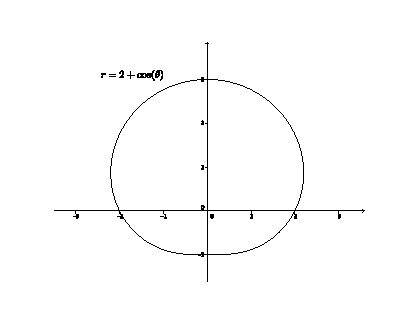
\includegraphics[width=0.6\textwidth]{WS6-1a}
\end{center}

 \item $r=\cos(2\theta)$, $\theta\in [0,2\pi]$

\begin{center}
 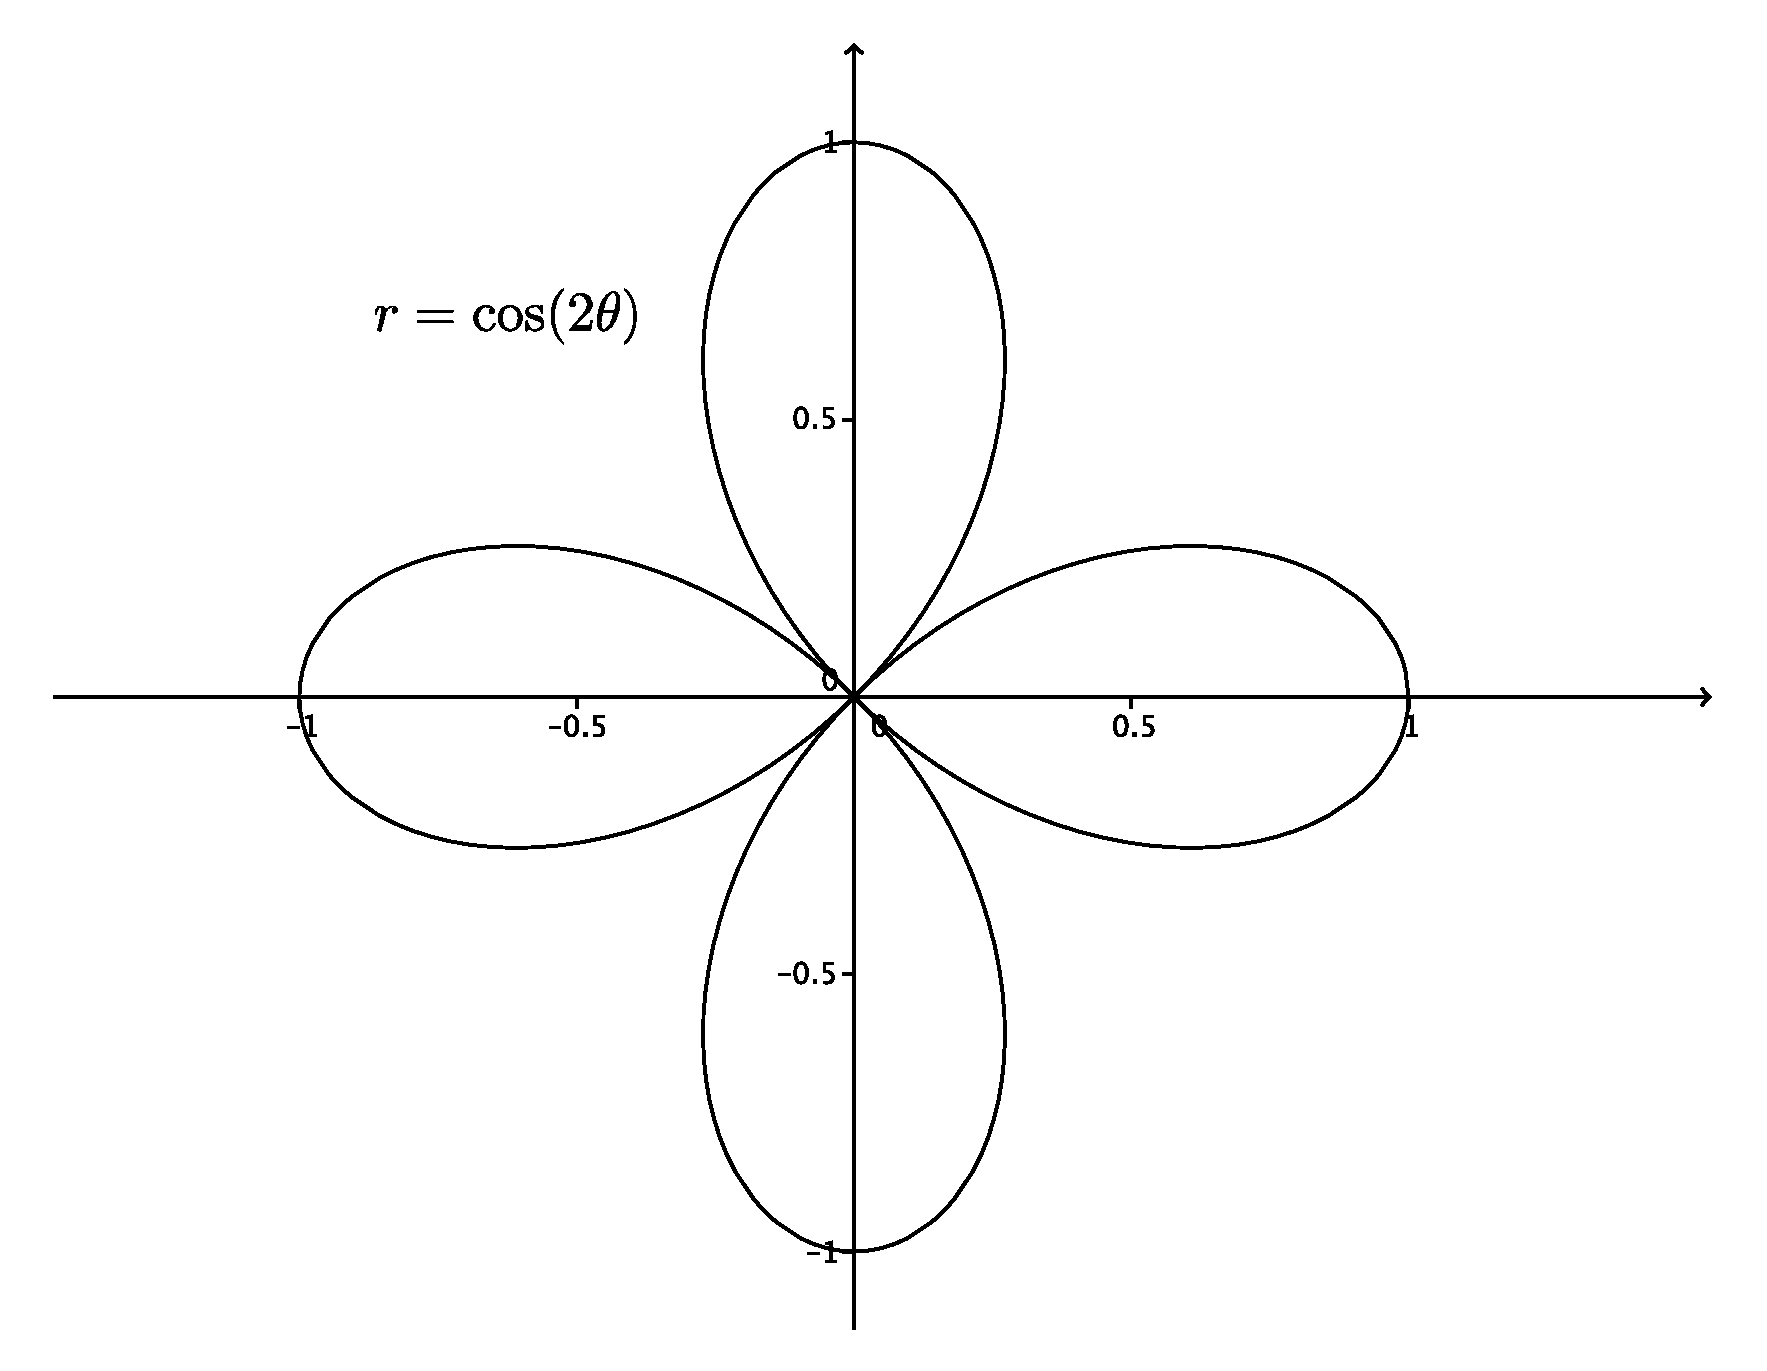
\includegraphics[width=0.6\textwidth]{WS6-1b}
\end{center}

 \item $r=2\cos(\theta)$, $\theta\in [-\pi/2,\pi/2]$

\begin{center}
 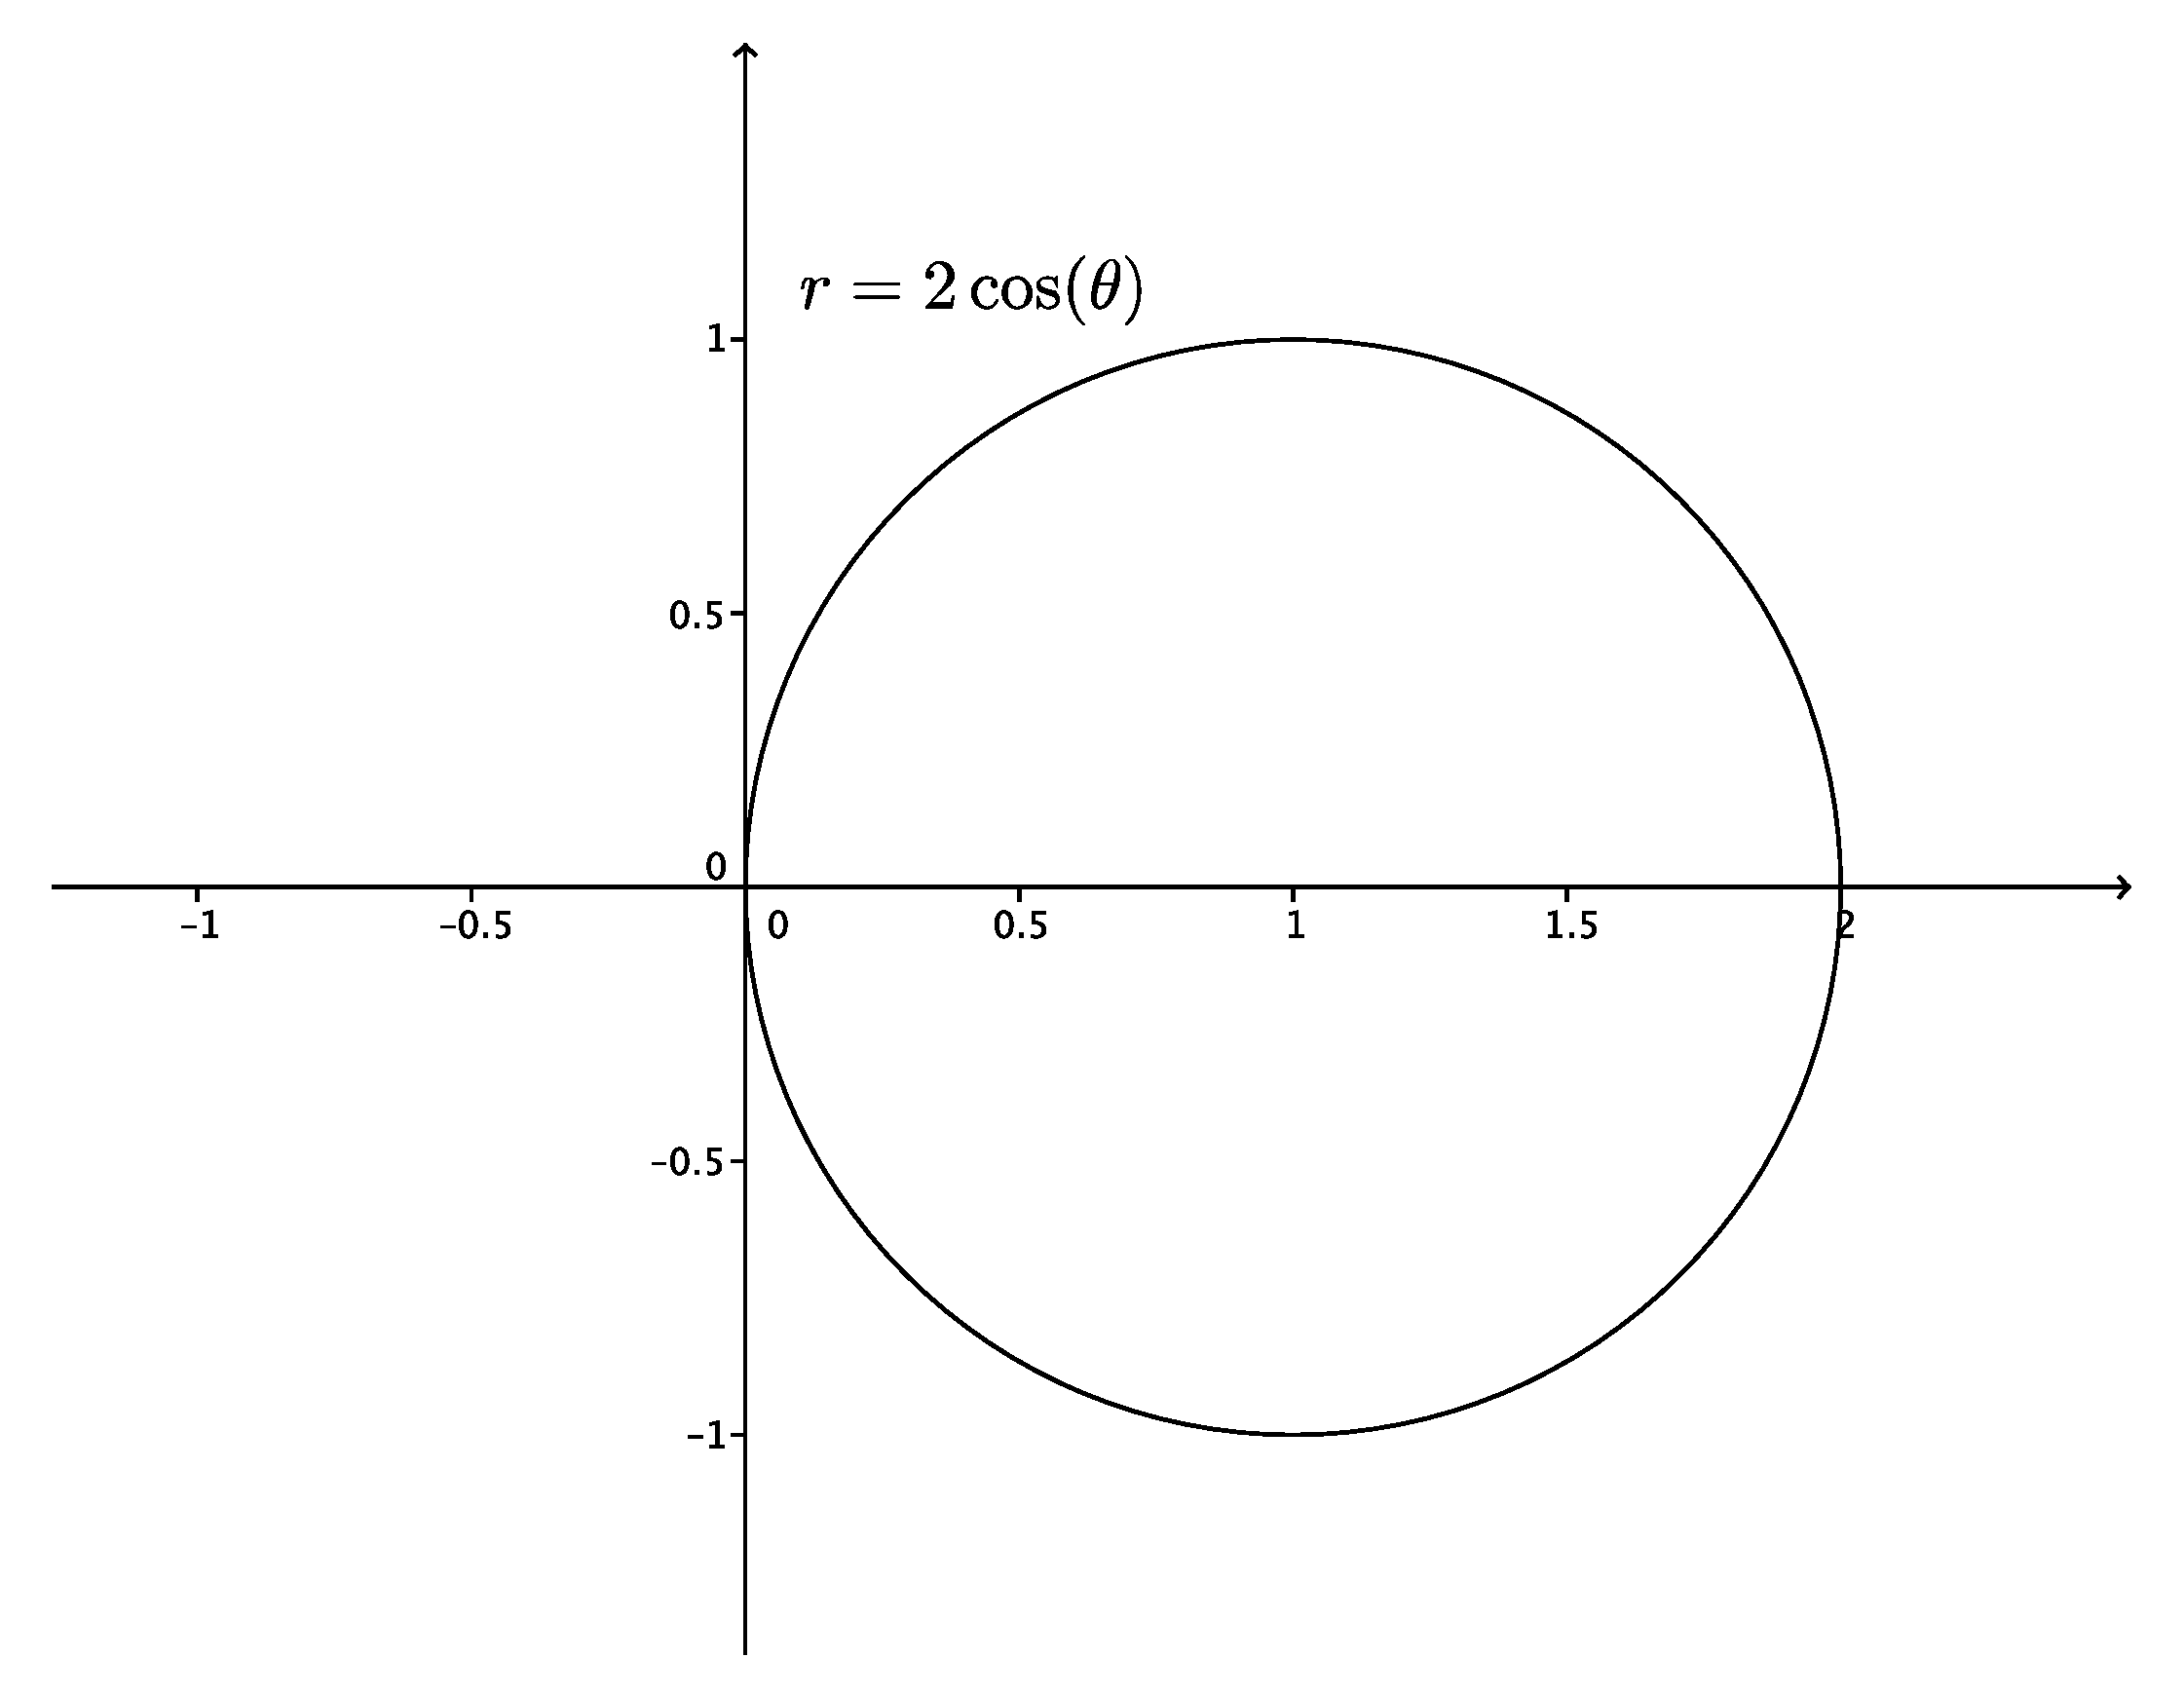
\includegraphics[width=0.6\textwidth]{WS6-1c}
\end{center}

Note that this is indeed a circle: if $r=2\cos\theta$, then $r^2=2r\cos\theta$, so $x^2+y^2=2x$. Completing the square gives $(x-1)^2+y^2=1$.

 \item $r^2=\cos(2\theta)$, $\theta\in [-\pi/4,\pi/4]\cup [3\pi/4, 5\pi/4]$

\begin{center}
 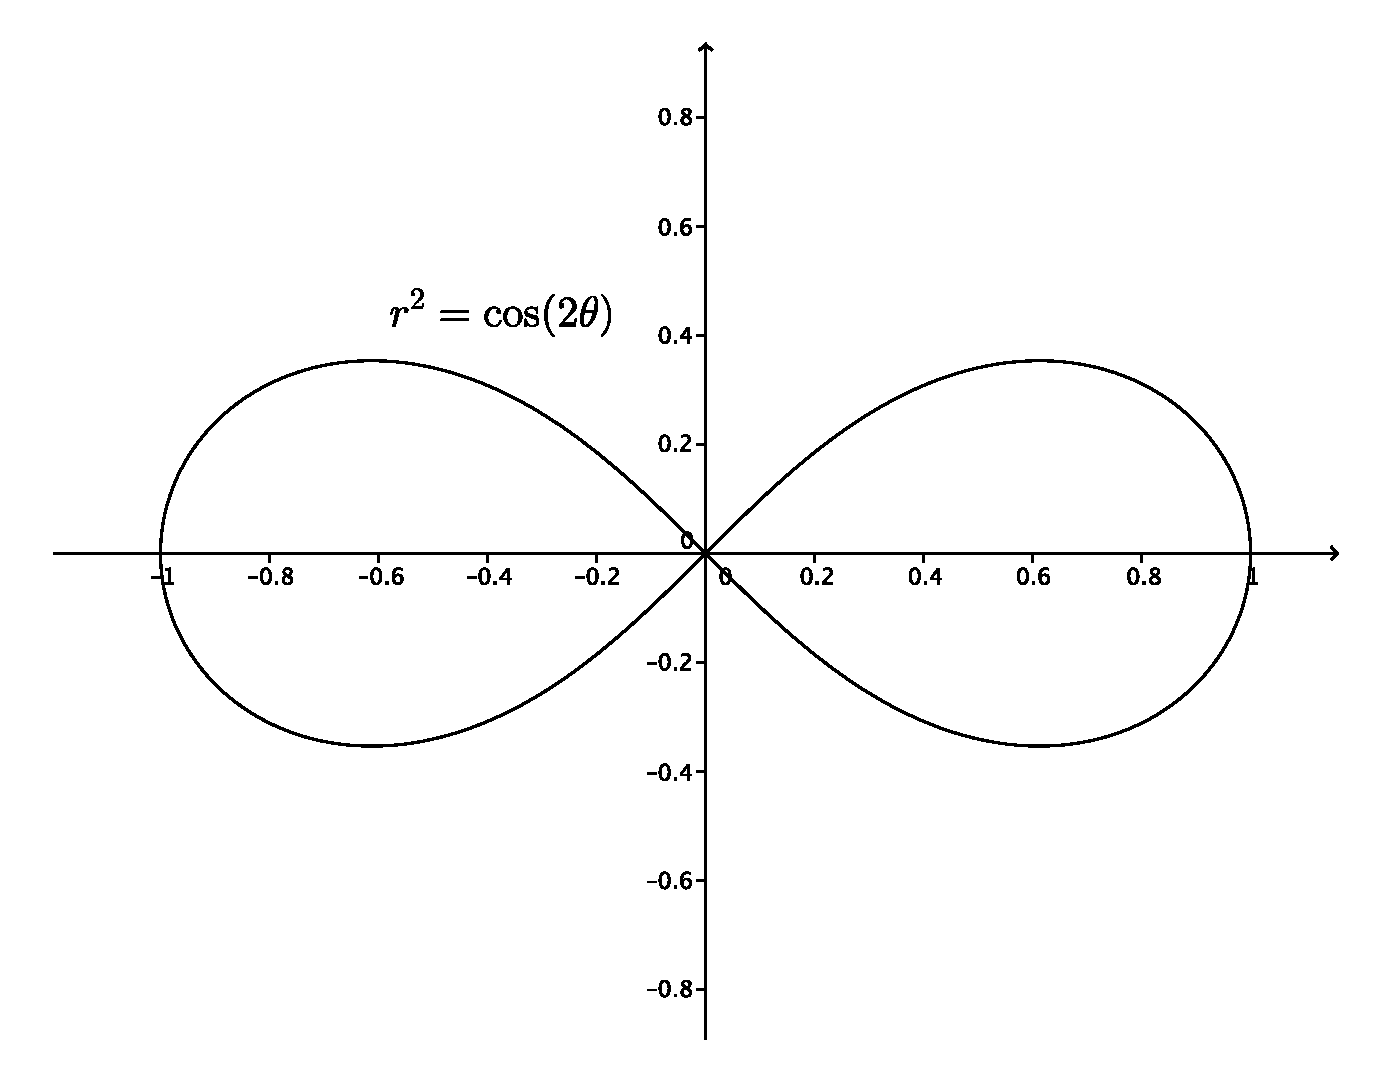
\includegraphics[width=0.6\textwidth]{WS6-1d}
\end{center}

\end{enumerate}
 \item Convert the polar equation to rectangular coordinates, and then plot:
\begin{enumerate}
 \item $r=\dfrac{3}{5\sin\theta -\cos\theta}$, $\theta\in [0,2\pi]$

\bigskip

Cross-multiplying gives us $3=5r\sin\theta-r\cos\theta = 5y-x$, so this is the line $5y-x=3$, with $x$-intercept $(-3,0)$ and $y$-intercept $(0,3/5)$. What's not so easy to see is that we do indeed get every point on the line. Note that the denominator of the original function of $\theta$ vanishes when $5\sin\theta-\cos\theta=0$, or $\tan\theta=\frac{1}{5}$. If we let $\alpha=\tan^{-1}(1/5)$, then as $\theta\to \alpha^-$, we have $r\to -\infty$, and as $\theta\to \alpha^+$, we have $r\to \infty$. 

In fact, for $\theta\in [0,2\pi]$, we start at the point $(3,0)$, when $\theta=0$. As $\theta$ increases from 0 to $\alpha$, we travel down (and to the left) along the line, since $r\to -\infty$. When $\theta=\alpha$, $r$ is undefined, but when we cross to $\theta>\alpha$, we suddenly jump to the other end of the line, off to the top right, since $r$ is very large and positive for values of $\theta>\alpha$ close to $\alpha$. As $r$ increase from $\alpha$ to $\pi$, we travel back down the line, passing through $(0,3/5)$ when $\theta=\pi/2$ and arriving again at the point $(-3,0)$ when $\theta=\pi$. Now, we note that if we let $\beta$ be the angle in the third quadrant where $\tan\beta = 1/5$ (that is, $\beta = \alpha+\pi$), we again have $r\to -\infty$ as $\theta\to \beta^-$, so we head back down the line again. 

Finally, we again jump to the other end of the line (where $x,y\to +\infty$) as we cross the point $\theta=\beta$, and then travel back down the line, reaching the point $(-3,0)$ one last time as $\theta$ reaches $2\pi$. So overall, we see the point $(-3,0)$ three times, and every other point on the line twice.


 \item $r=3\sec\theta$, $\theta\in (-\pi/2,\pi/2)$

\bigskip

We have $r=3\sec\theta = \dfrac{3}{\cos\theta}$, so $r\cos\theta=3$, giving us the vertical line $x=3$. Again, we note that $r\to \infty$ as $\theta\to \pi/2^+$, and $r\to-\infty$ as $\theta\to -\pi/2^-$, so we traverse the entire line $x=3$ over the given interval.

 \item $\theta = \pi/6$

\bigskip

The equation $\theta=\pi/6$ describes the ray beginning from the origin and travelling outward along the line which makes an angle of $\pi/6$ with the $x$-axis. To recover the equation of this line, note that when $\theta=\pi/6$, we have $x=r\cos(\pi/6) = \dfrac{\sqrt{3}{2}}r$, and $y=r\sin(\pi/6) = \frac{1}{2}r$. Thus, $\dfrac{x}{y}=\sqrt{3}$, or $x=\sqrt{3}y$.

\end{enumerate}
 \item Find the points of intersection of the polar curves. (Note that the point $(0,0)$ requires special care: you might have $r=0$ for \textit{different} values of $\theta$ for the two curves.)
\begin{enumerate}
 \item $r=\cos(2\theta)$ and $r=\cos\theta$, on $[0,2\pi]$

\bigskip

To help us be sure we've found all the points of intersection, we plot the two curves:

\begin{center}
 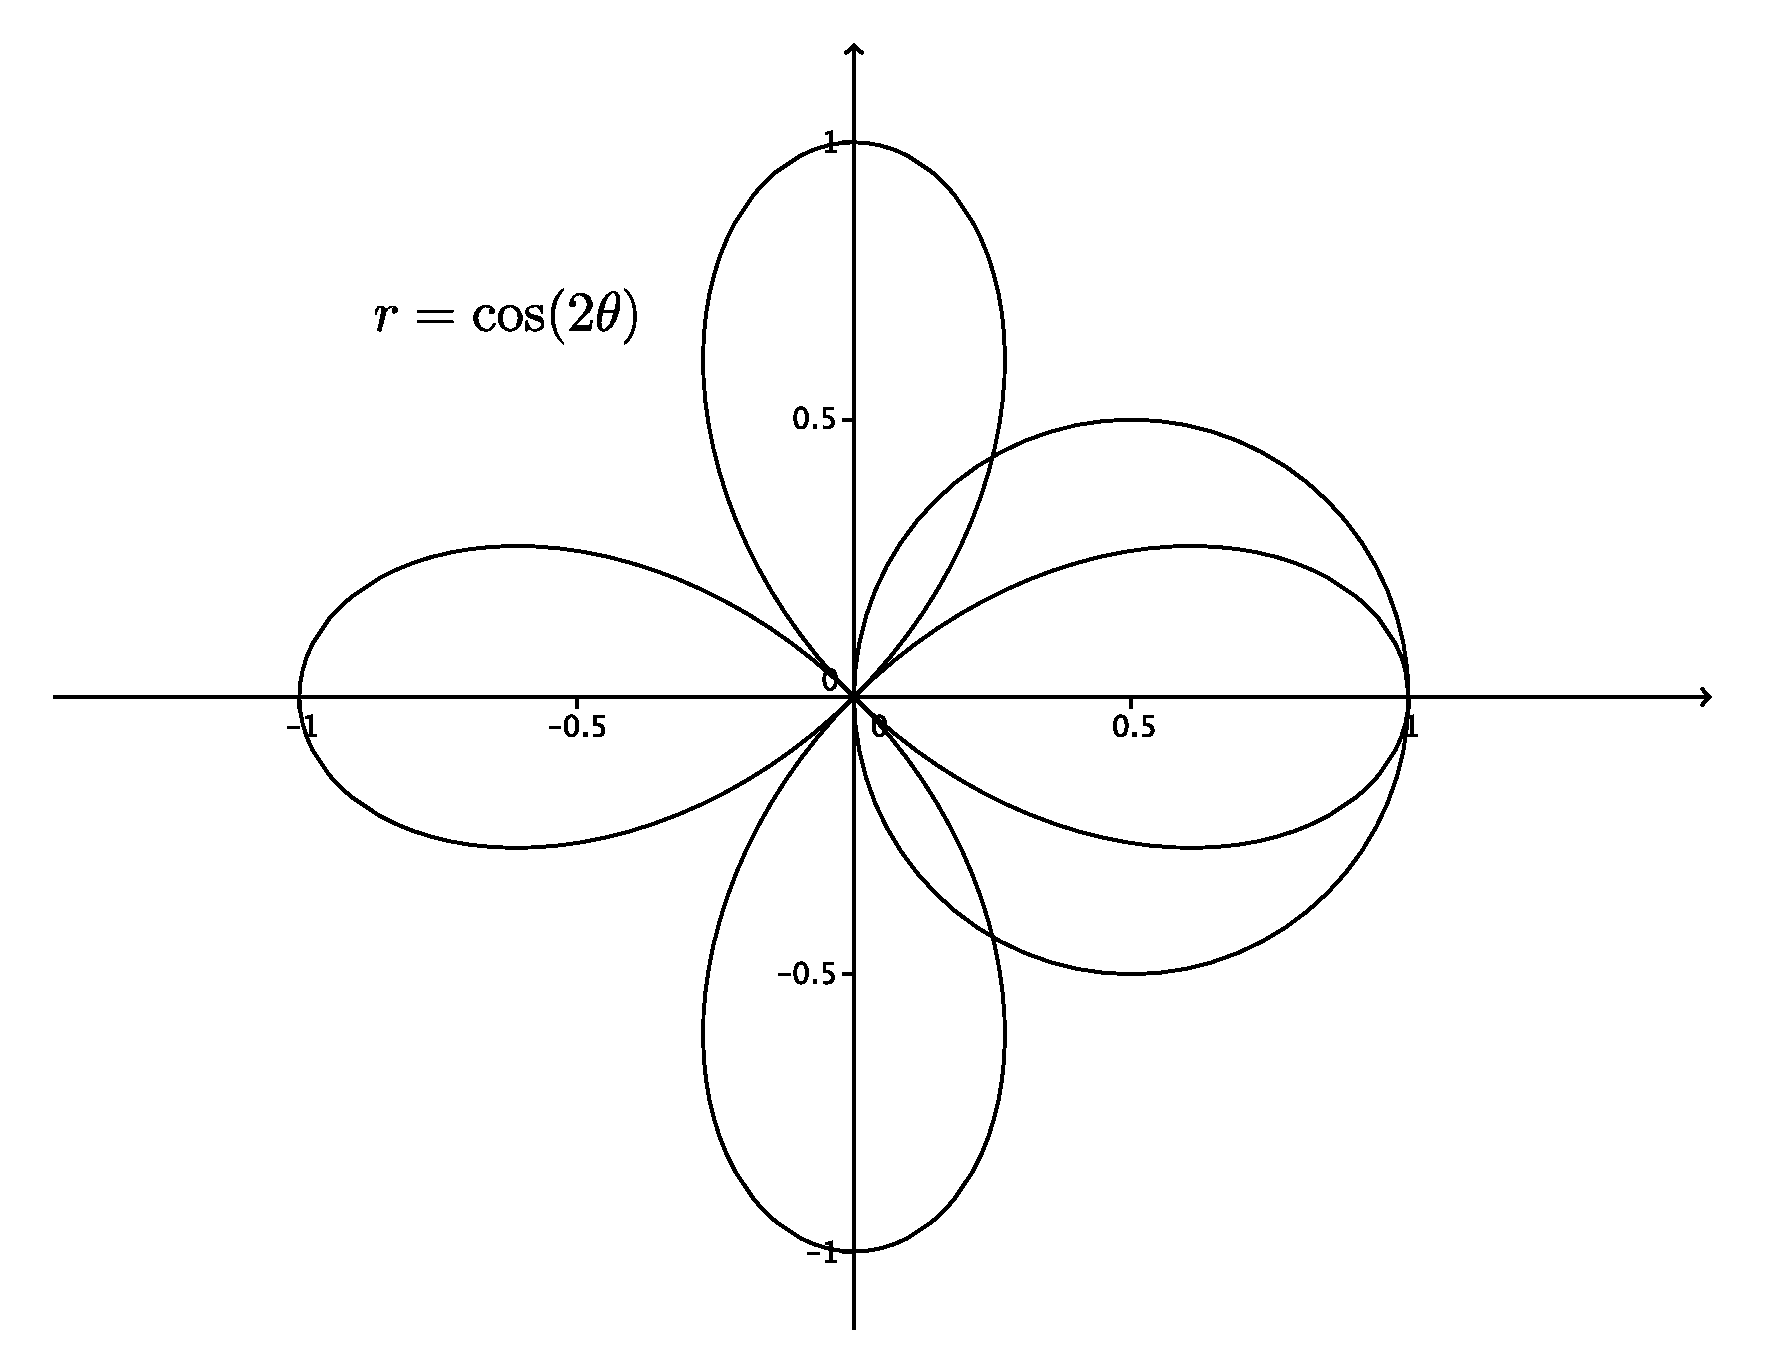
\includegraphics[width=0.6\textwidth]{WS6-3a}
\end{center}

From the plot, we see that there should be four points of intersection, and one of the points is the origin. The origin is given by $r=0$, for \textbf{any} value of $\theta$. (This is the one drawback of polar coordinates: we have one point that does not determine a unique set of values for $r$ and $\theta$. (OK, technically this is true of all points, since we can always add $2\pi$ to $\theta$, but we can always restrict the interval for $\theta$.))

For the curve $r=\cos(2\theta)$, $r=0$ gives $\cos(2\theta)=0$, so $2\theta$ must be an odd multiple of $\pi/2$. On the interval $[0,2\pi]$, this happens for $\theta = \pi/4, 3\pi/4, 5\pi/4$, and $7\pi/4$. On the other hand, setting $r=0$ in the equation $r=\cos\theta$ gives us $\theta = \pi/2$ or $\theta = 3\pi/2$. Even though none of the $\theta$ values agree, $(0,0)$ is nonetheless a point of intersection.

Now, for the other points of intersection, $r\neq 0$, so we must have $\cos(2\theta)=\cos(\theta)$. Since $\cos(2\theta) = 2\cos^2\theta-1$, we get $2\cos^2(\theta)-1=\cos(theta)$, or $2\cos^2\theta-\cos(\theta)-1 = (2\cos(\theta)+1)(\cos\theta-1)=0$. Thus, either $\cos\theta = -\dfrac{1}{2}$, giving us either $\theta = 2\pi/3$ or $\theta = 4\pi/3$, or $\cos\theta = 1$, giving us $\theta=0$ or $\theta = 2\pi$.

Using the curve $r=\cos(\theta)$, we have $x=\cos^2\theta$ and $y=\cos\theta\sin\theta$. When $\theta = 2\pi/3$, we have $x=\left(\frac{-1}{2}\right)^2 = \frac{1}{4}$ and $y = -\frac{1}{2}\cdot \frac{\sqrt{3}{2}} = -\frac{\sqrt{3}}{4}$, so this is the point of intersection below the $y$-axis seen above. Similarly, when $\theta = 4\pi/3$, we get $x=\frac{1}{4}$ and $y = \frac{\sqrt{3}}{4}$, so this is the point of intersection above the $y$-axis. Finally, putting $\theta=0$ (or $2\pi$) gives us the point of intersection $(1,0)$.


 \item $r=\sin\theta$ and $r=\sqrt{3}+3\sin\theta$, on $[0,2\pi]$

From the plot below, we see that there are three points of intersection: one at the origin, and one in each of the first and second quadrants.


\begin{center}
 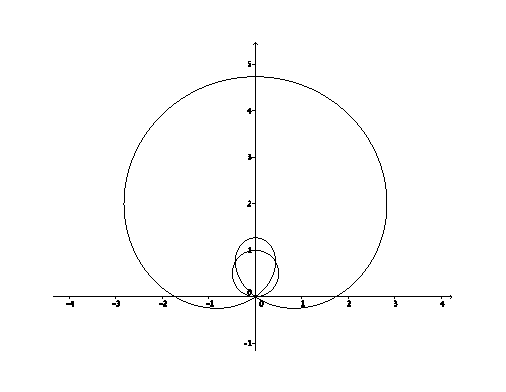
\includegraphics[width=0.6\textwidth]{WS6-3b}
\end{center}

As above, we confirm the intesection at the origin as a special case. The first curve passes through the origin for $\theta = 0, \pi, 2\pi$, and the other when $\sin(\theta) = -\dfrac{1}{\sqrt{3}}$. For the other two points of intersection, we set $\sin\theta = \sqrt{3}+3\sin\theta$, giving us $\sin\theta = -\dfrac{\sqrt{3}}{2}$, so $\theta = 4\pi/3$ or $\theta = 5\pi/3$. Using $r=\sin\theta$, we have $x = \sin\theta\cos\theta$ and $y=\sin^2\theta$. When $\theta = 4\pi/3$, we have $x=(-\sqrt{3}/2)(-1/2) = \sqrt{3}/4$, while $y = (\sqrt{3}/2)^2 = 3/4$. Thus, the point of intersection in the first quadrant is $\left(\frac{\sqrt{3}{4}},\frac{3}{4}\right)$. Similarly, we find that the point of intersection in the second quadrant is $\left(\frac{-\sqrt{3}}{4},\frac{3}{4}\right)$.

 \item $r=1-\cos\theta$ and $r=1+\sin\theta$ on $[0,2\pi]$

From the graph below, we see that there are three points of intersection: one at the origin, one in the second quadrant, and one in the fourth quadrant.

\begin{center}
 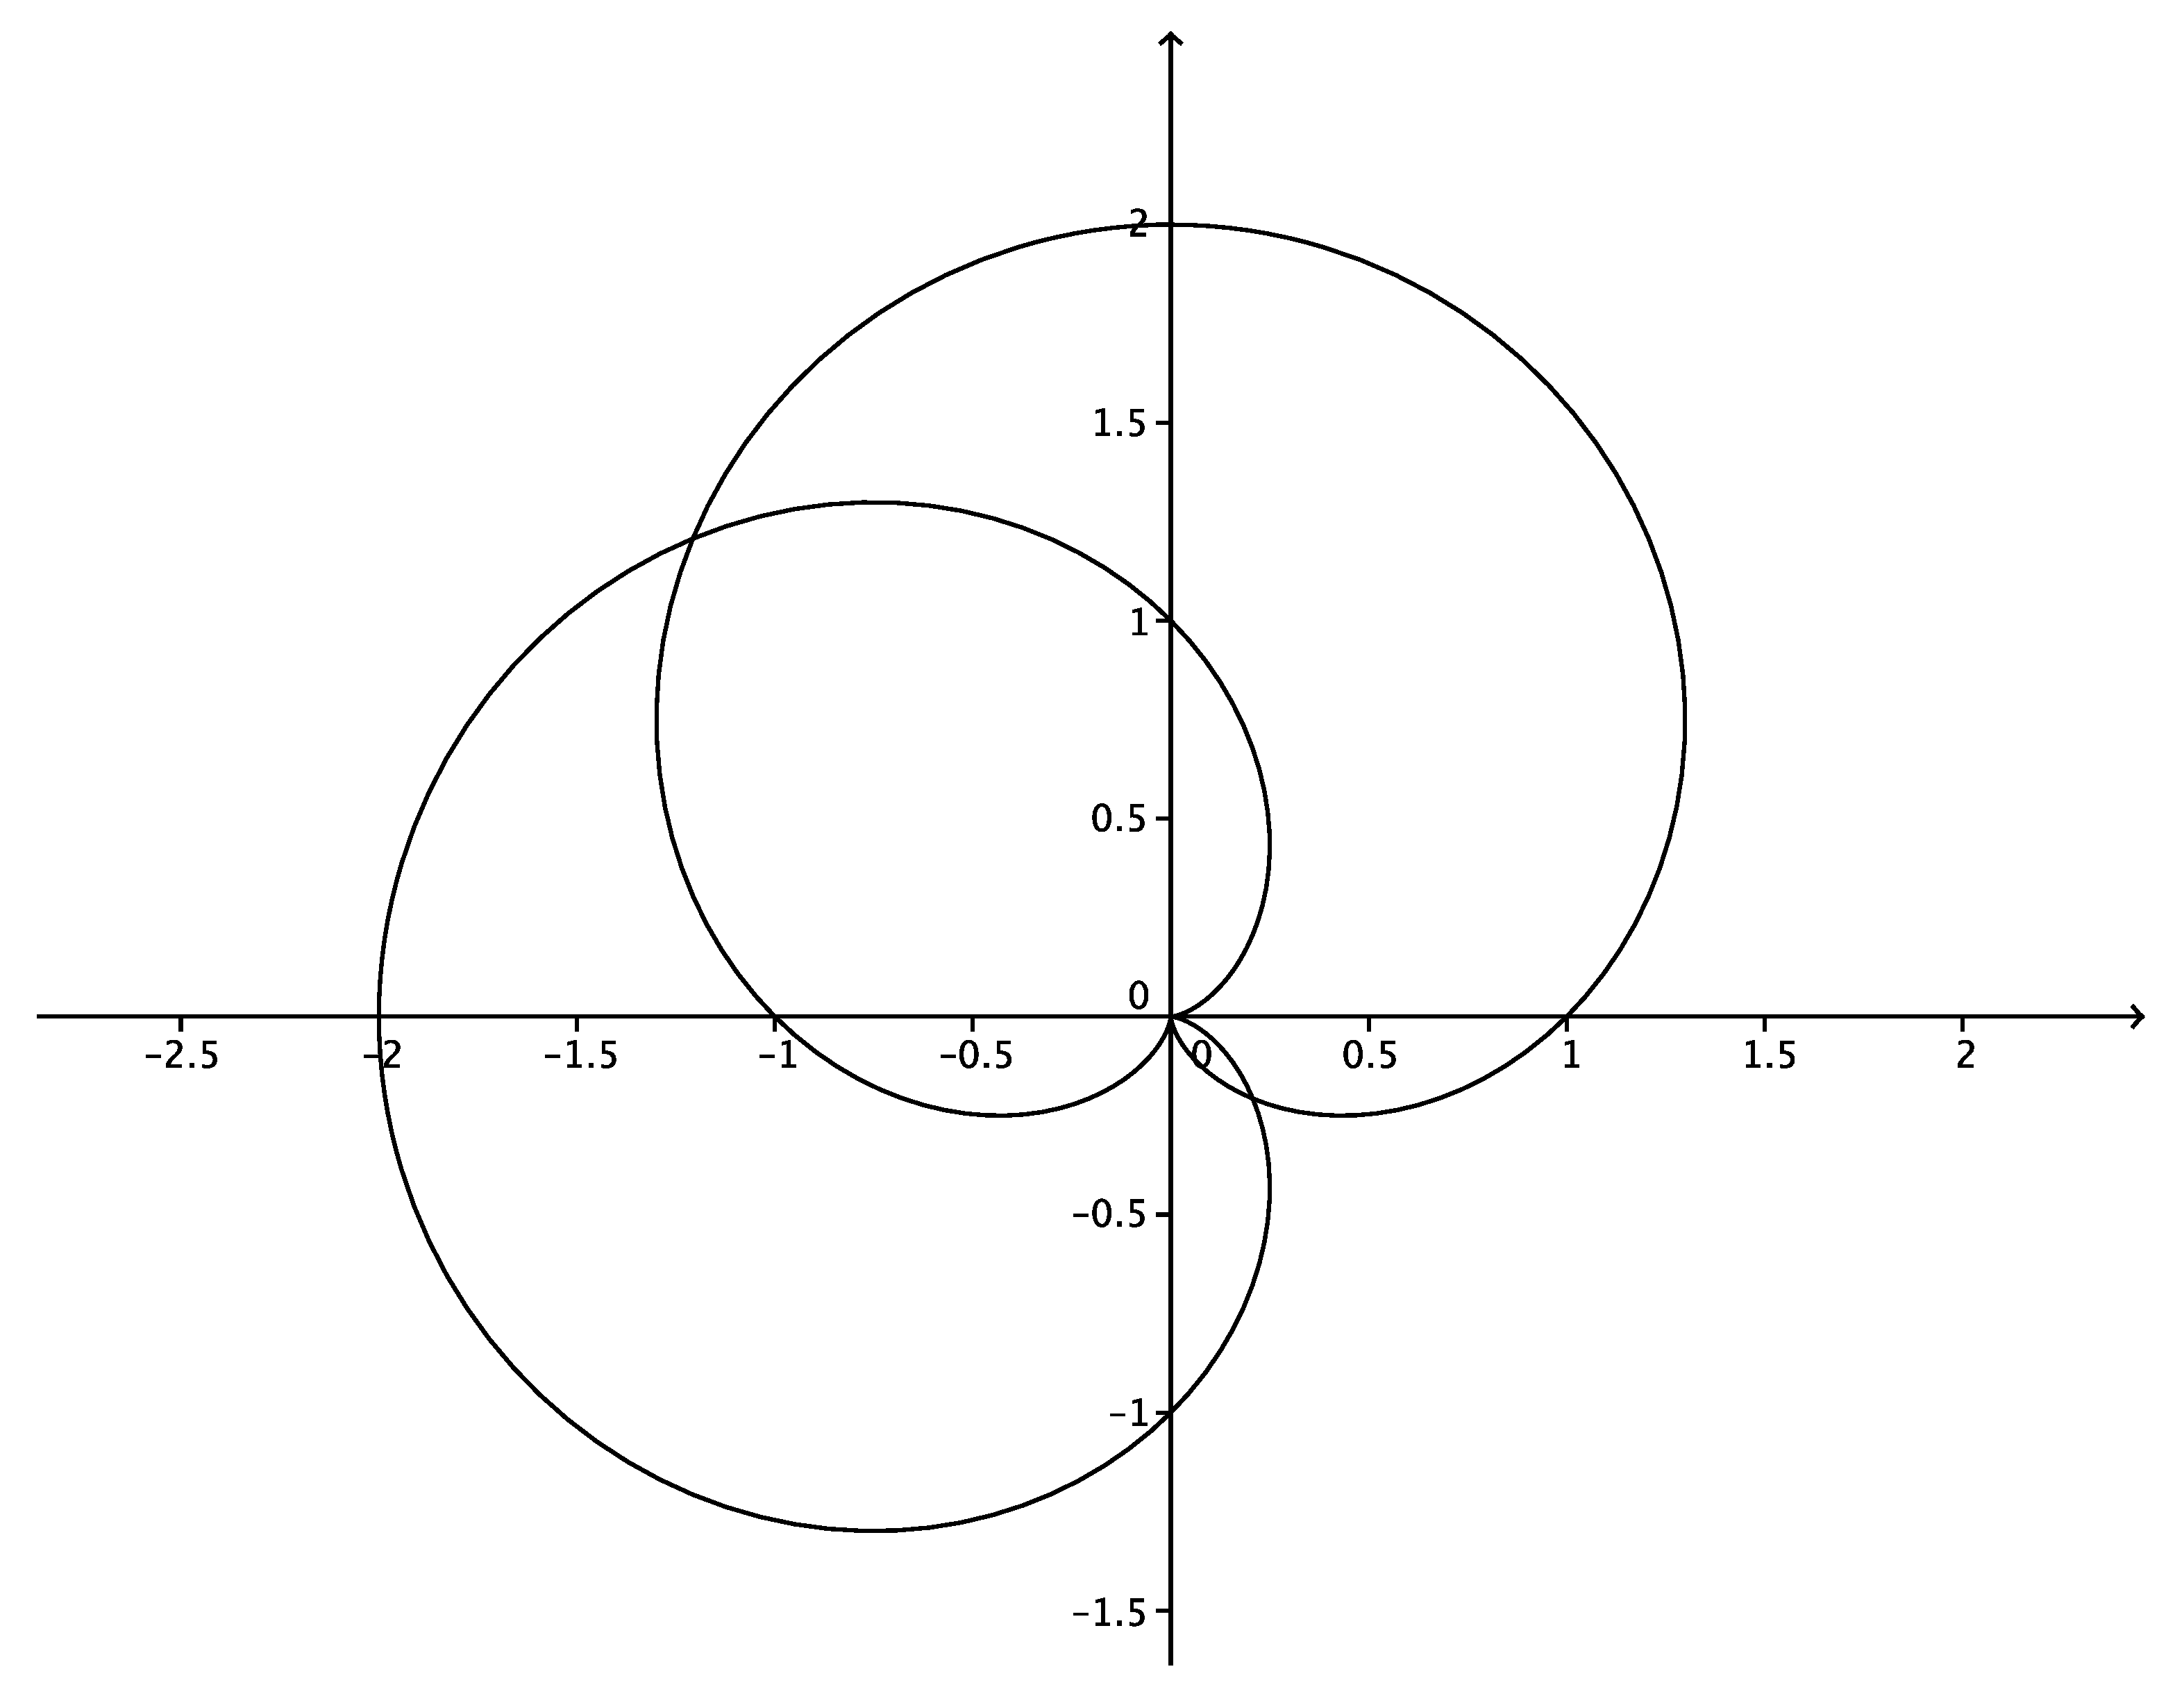
\includegraphics[width=0.6\textwidth]{WS6-3c}
\end{center}

I'll leave it for you to verify that both curves do indeed pass through the origin. For the other two points of intersection, we set $1-\cos\theta=1+\sin\theta$, which can be rewritten as $\tan\theta = -1$. For $\theta\in [0,2\pi]$ we thus have either $\theta = 3\pi/4$ or $\theta = 7\pi/4$. Using the $r=1-\cos\theta$, we have $x=\cos\theta-\cos^2\theta$ and $y = \sin\theta-\sin\theta\cos\theta$. If $\theta = 3\pi/4$, we have $x=-\dfrac{(1+\sqrt{2})}{2}$, and $y=\dfrac{1+\sqrt{2}}{2}$. This is the point of intersection in the second quadrant. If $\theta = 7\pi/4$, we have $x=\dfrac{\sqrt{2}-1}{2}$ and $y=\dfrac{1-\sqrt{2}}{2}$. This is the point of intersection in the fourth quadrant.

 \item $r=\cos(3\theta)$ and $r=\sin(3\theta)$, on $[0,2\pi]$


\begin{center}
 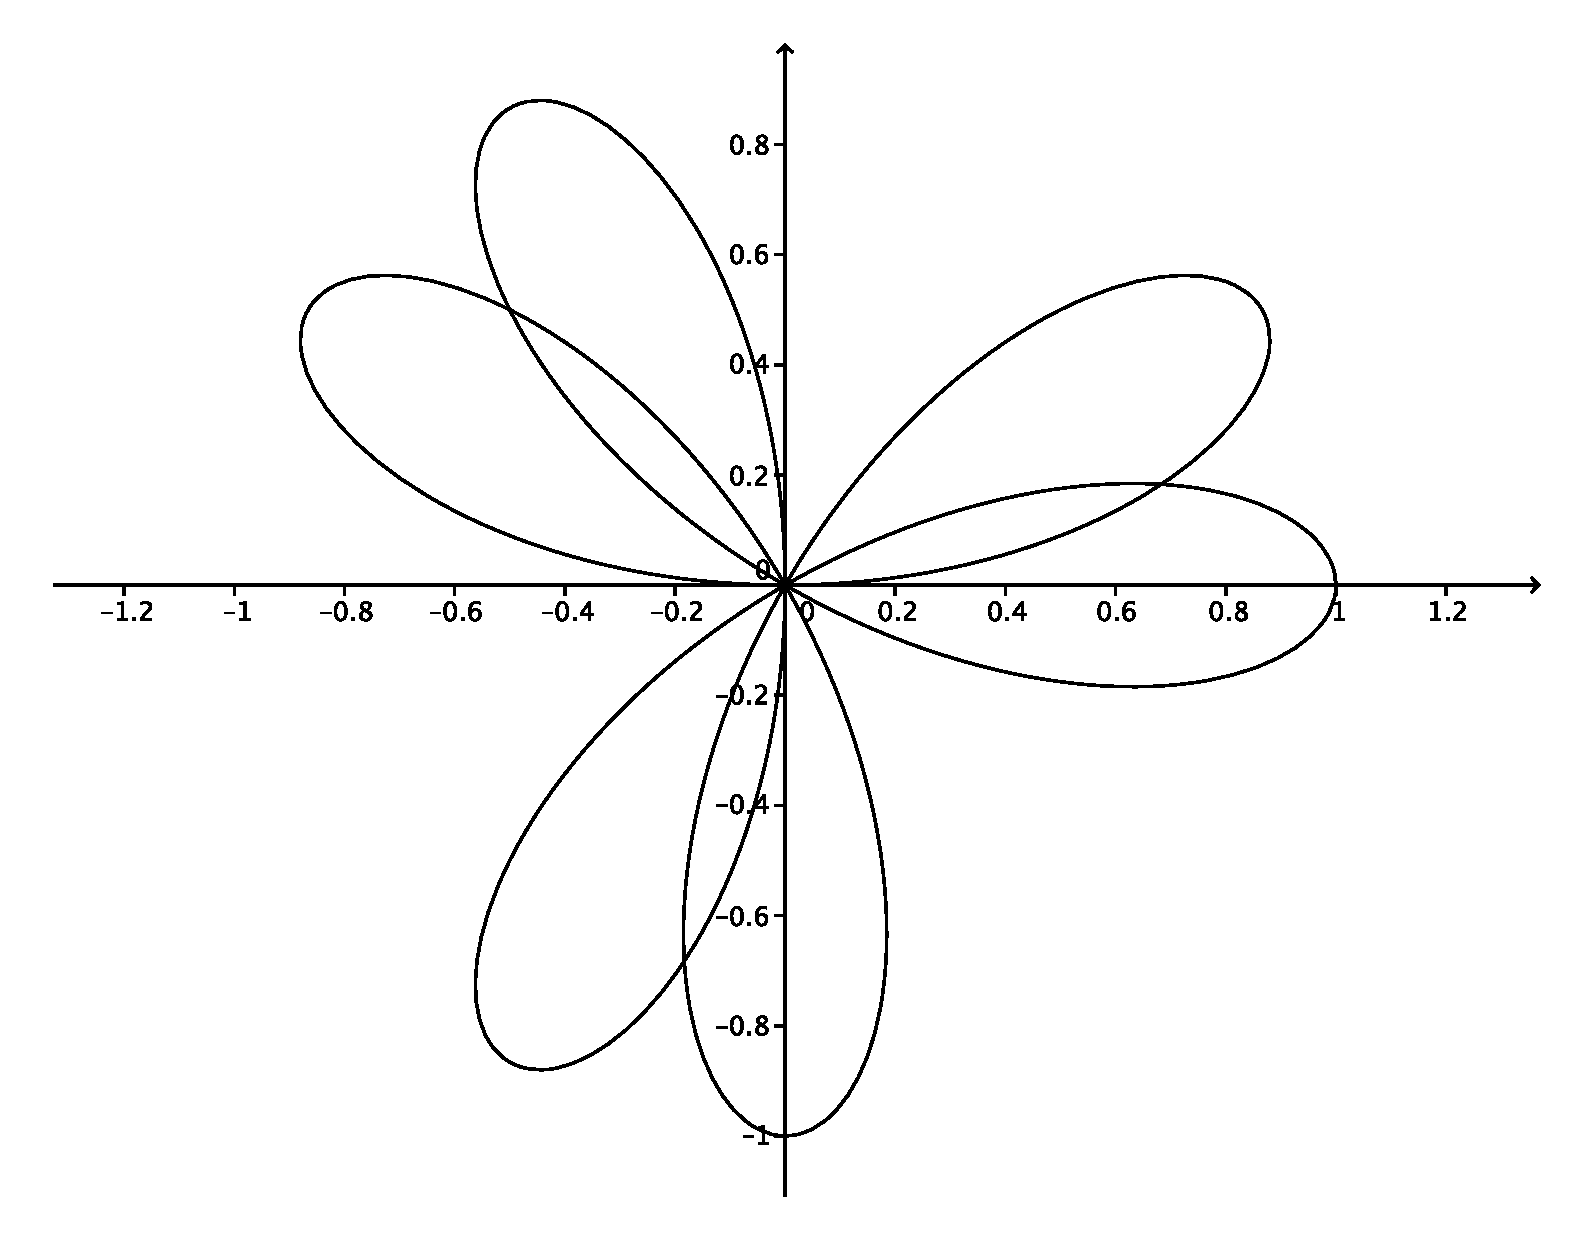
\includegraphics[width=0.6\textwidth]{WS6-3d}
\end{center}

From the graph we can see that both curves intersect at the origin (many times), and that there are three other points of intersection, in the first, second and third quadrants. Setting $\cos(3\theta)=\sin(3\theta)$, we get $\tan(3\theta) = 1$, so we must have $3\theta = \pi/4$ or $3\theta = 5\pi/4$. For $\theta\in [0,2\pi]$, this gives us the following possibilities: $\theta = \pi/12, 5\pi/12, 9\pi/12 = 3\pi/4, 13\pi/12, 17\pi/12$, and $21\pi/12 = 7\pi/3$. However, the first three values of $\theta$ suffice: you can check that the other three values simply repeat the same three points of intersection.

I'll leave it to you to work out the $x$ and $y$ coordinates for each point of intersection.

\end{enumerate}
 \item Find the area enclosed by the following polar curves:
\begin{enumerate}
 \item One loop of the three-leaf rose $r=\sin(3\theta)$.


\begin{center}
 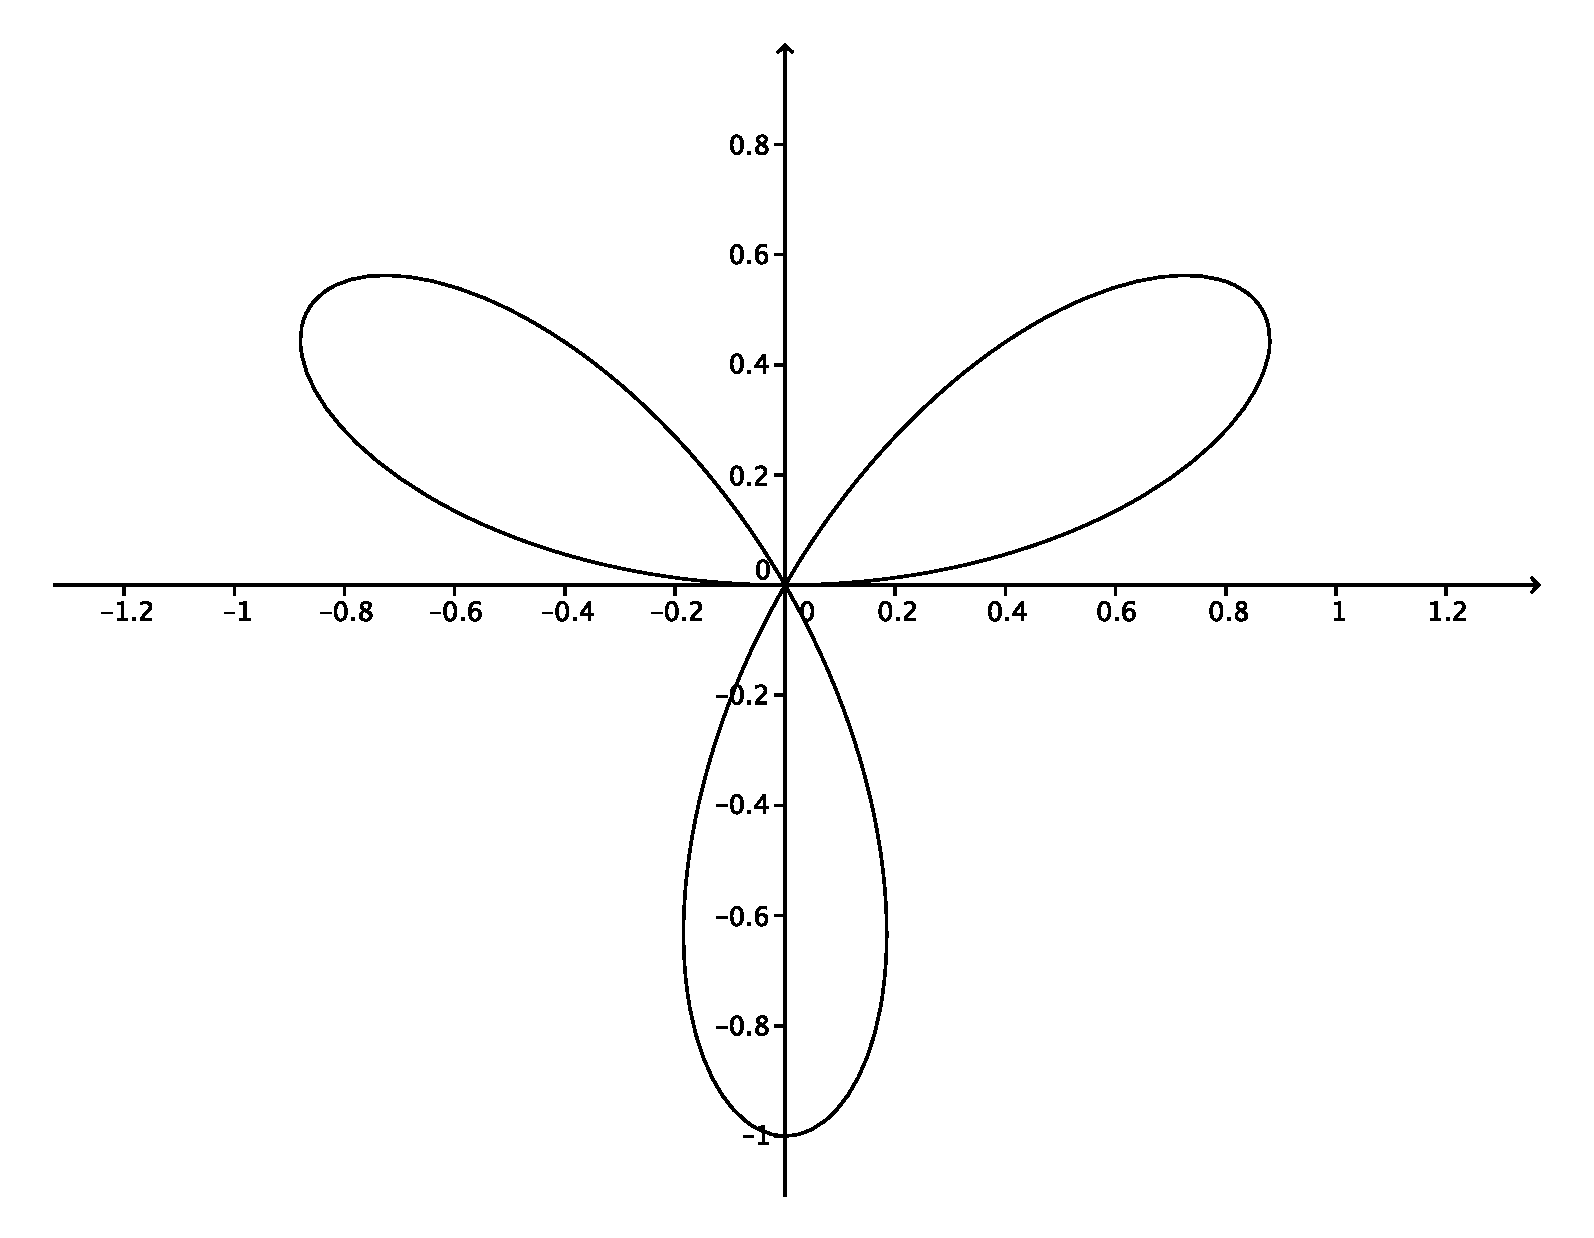
\includegraphics[width=0.6\textwidth]{WS6-4a}
\end{center} 

The three-leaf rose is pictured above. We'll find the area enclosed by the loop in the first quadrant. We note that $\sin(3(0))=0$, so the curve begins at the origin when $\theta=0$. As $\theta$ increases, we enter the first quadrant, and remain there until we reach $\sin(3\theta)=0$ again, which happens when $3\theta = \pi$, so $\theta = \pi/3$. Using the formula $\di A = \int_\alpha^\beta \frac{1}{2}r(\theta)^2\,d\theta$ for area, we thus have
\[
 A = \frac{1}{2}\int_0^{\pi/3}\sin^2(3\theta)\,d\theta = \frac{1}{4}\int_0^\pi/3 (1-\cos(6\theta))\,d\theta = \frac{1}{4}(\frac{\pi}{3}) = \frac{\pi}{12}.
\]

 \item The outer loop of the lima{\c c}on $r=1+2\cos\theta$.

\begin{center}
 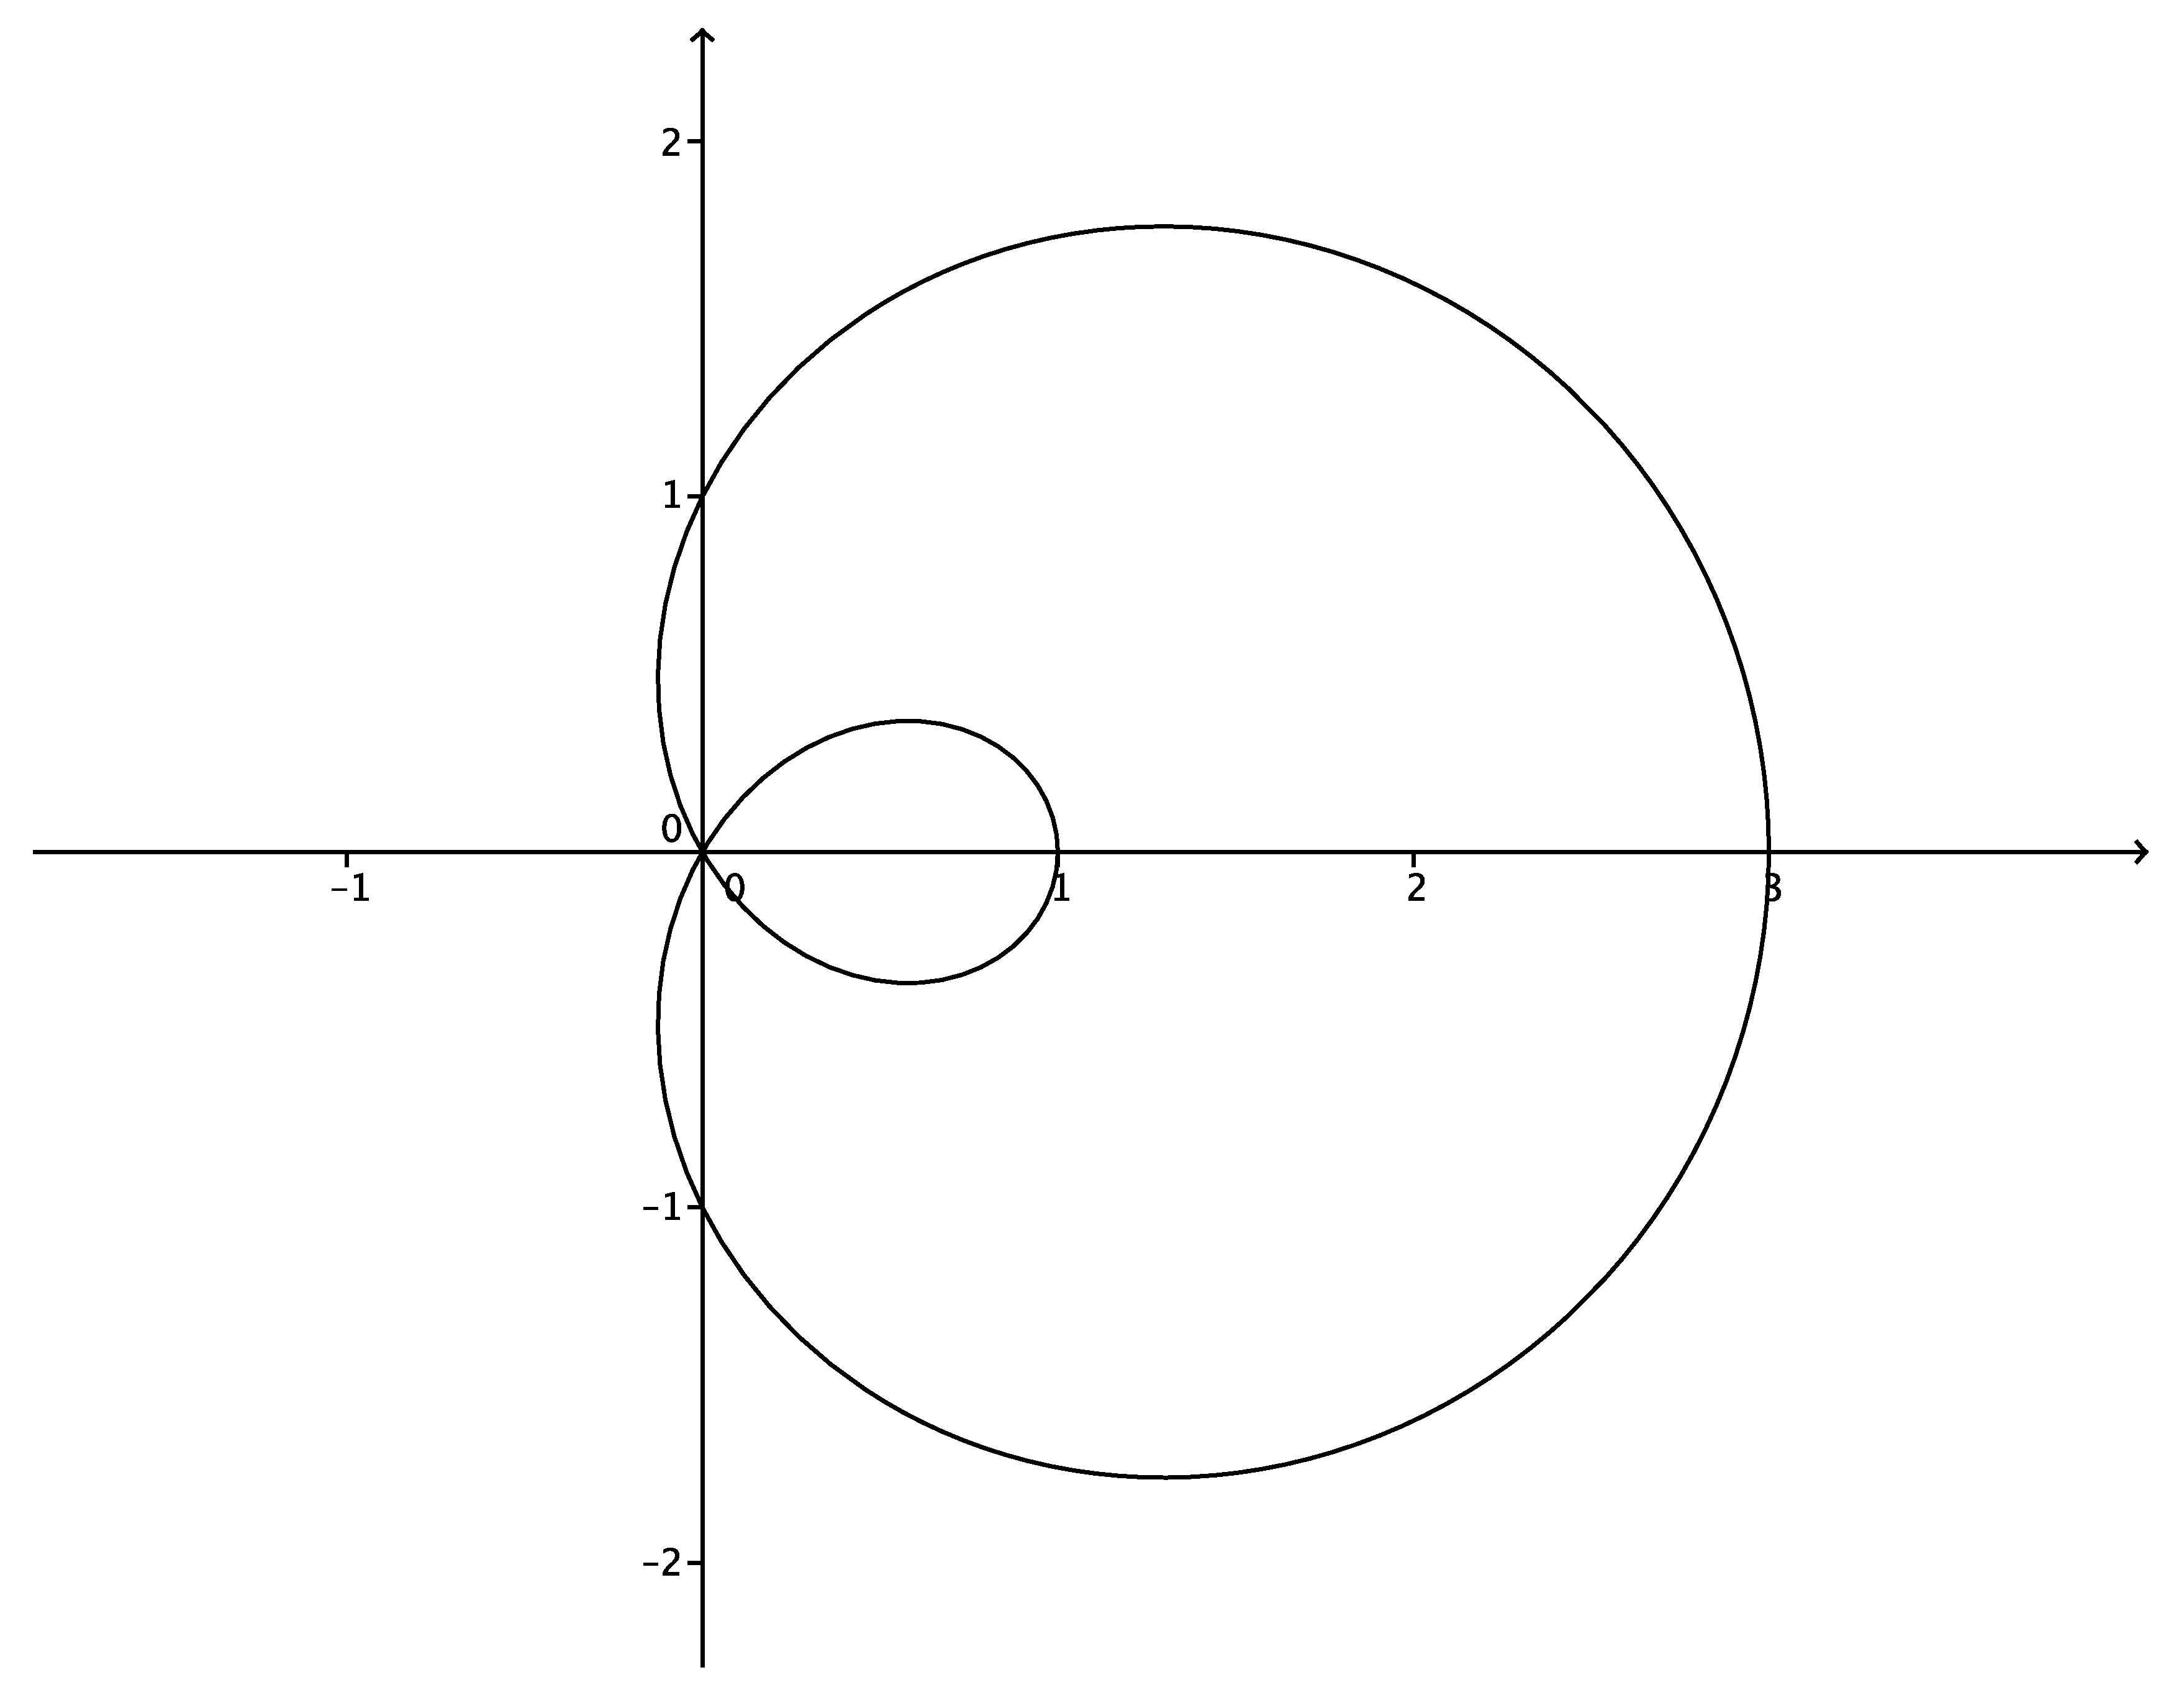
\includegraphics[width=0.6\textwidth]{WS6-4b}
\end{center}

There's a bit of interpretation required here: does ``enclosed by the outer loop'' mean everything inside the outer loop, or does it mean everything that is inside the outer loop, but outside the inner loop? It seems more likely that it means the former. If we start at $\theta = 0$, we begin at $(3,0)$ and trace out the top half of the loop, returning to the origin when $\cos\theta = -1/2$, or $\theta = 2\pi/3$. For $2\pi/3\leq \theta\leq 4\pi/3$ we trace out the inner loop, and from $4\pi/3$ to $2\pi$ we get the bottom of the outer loop. By symmetry, the desired area is twice the area between the upper half of the outer loop and the $x$-axis. Thus,
\begin{align*}
 A &= 2\int_0^{2\pi/3}\frac{1}{2}(1+2\cos\theta)^2\,d\theta = \int_0^{2\pi/3}(1+4\cos\theta+4\cos^2\theta)\,d\theta\\
& = \int_0^{2\pi/3}(3+4\cos\theta+2\cos(2\theta)\,d\theta = \left. 3\theta+4\sin\theta+\sin(2\theta)\right|_0^{2\pi/3}\\
& = 2\pi+\frac{3\sqrt{3}}{2}
\end{align*}

Note: if you don't invoke symmetry, it's a good idea to replace the interval $[0,2\pi]$ with the interval $[-\pi,\pi]$. Leaving out the inner loop means integrating from $-2\pi/3$ to $2\pi/3$ rather than integrating from 0 to $2\pi/3$ and then from $4\pi/3$ to $2\pi$.

 \item Inside the circle $r=2\cos\theta$, but outside the circle $r=2\sin\theta$.

\begin{center}
 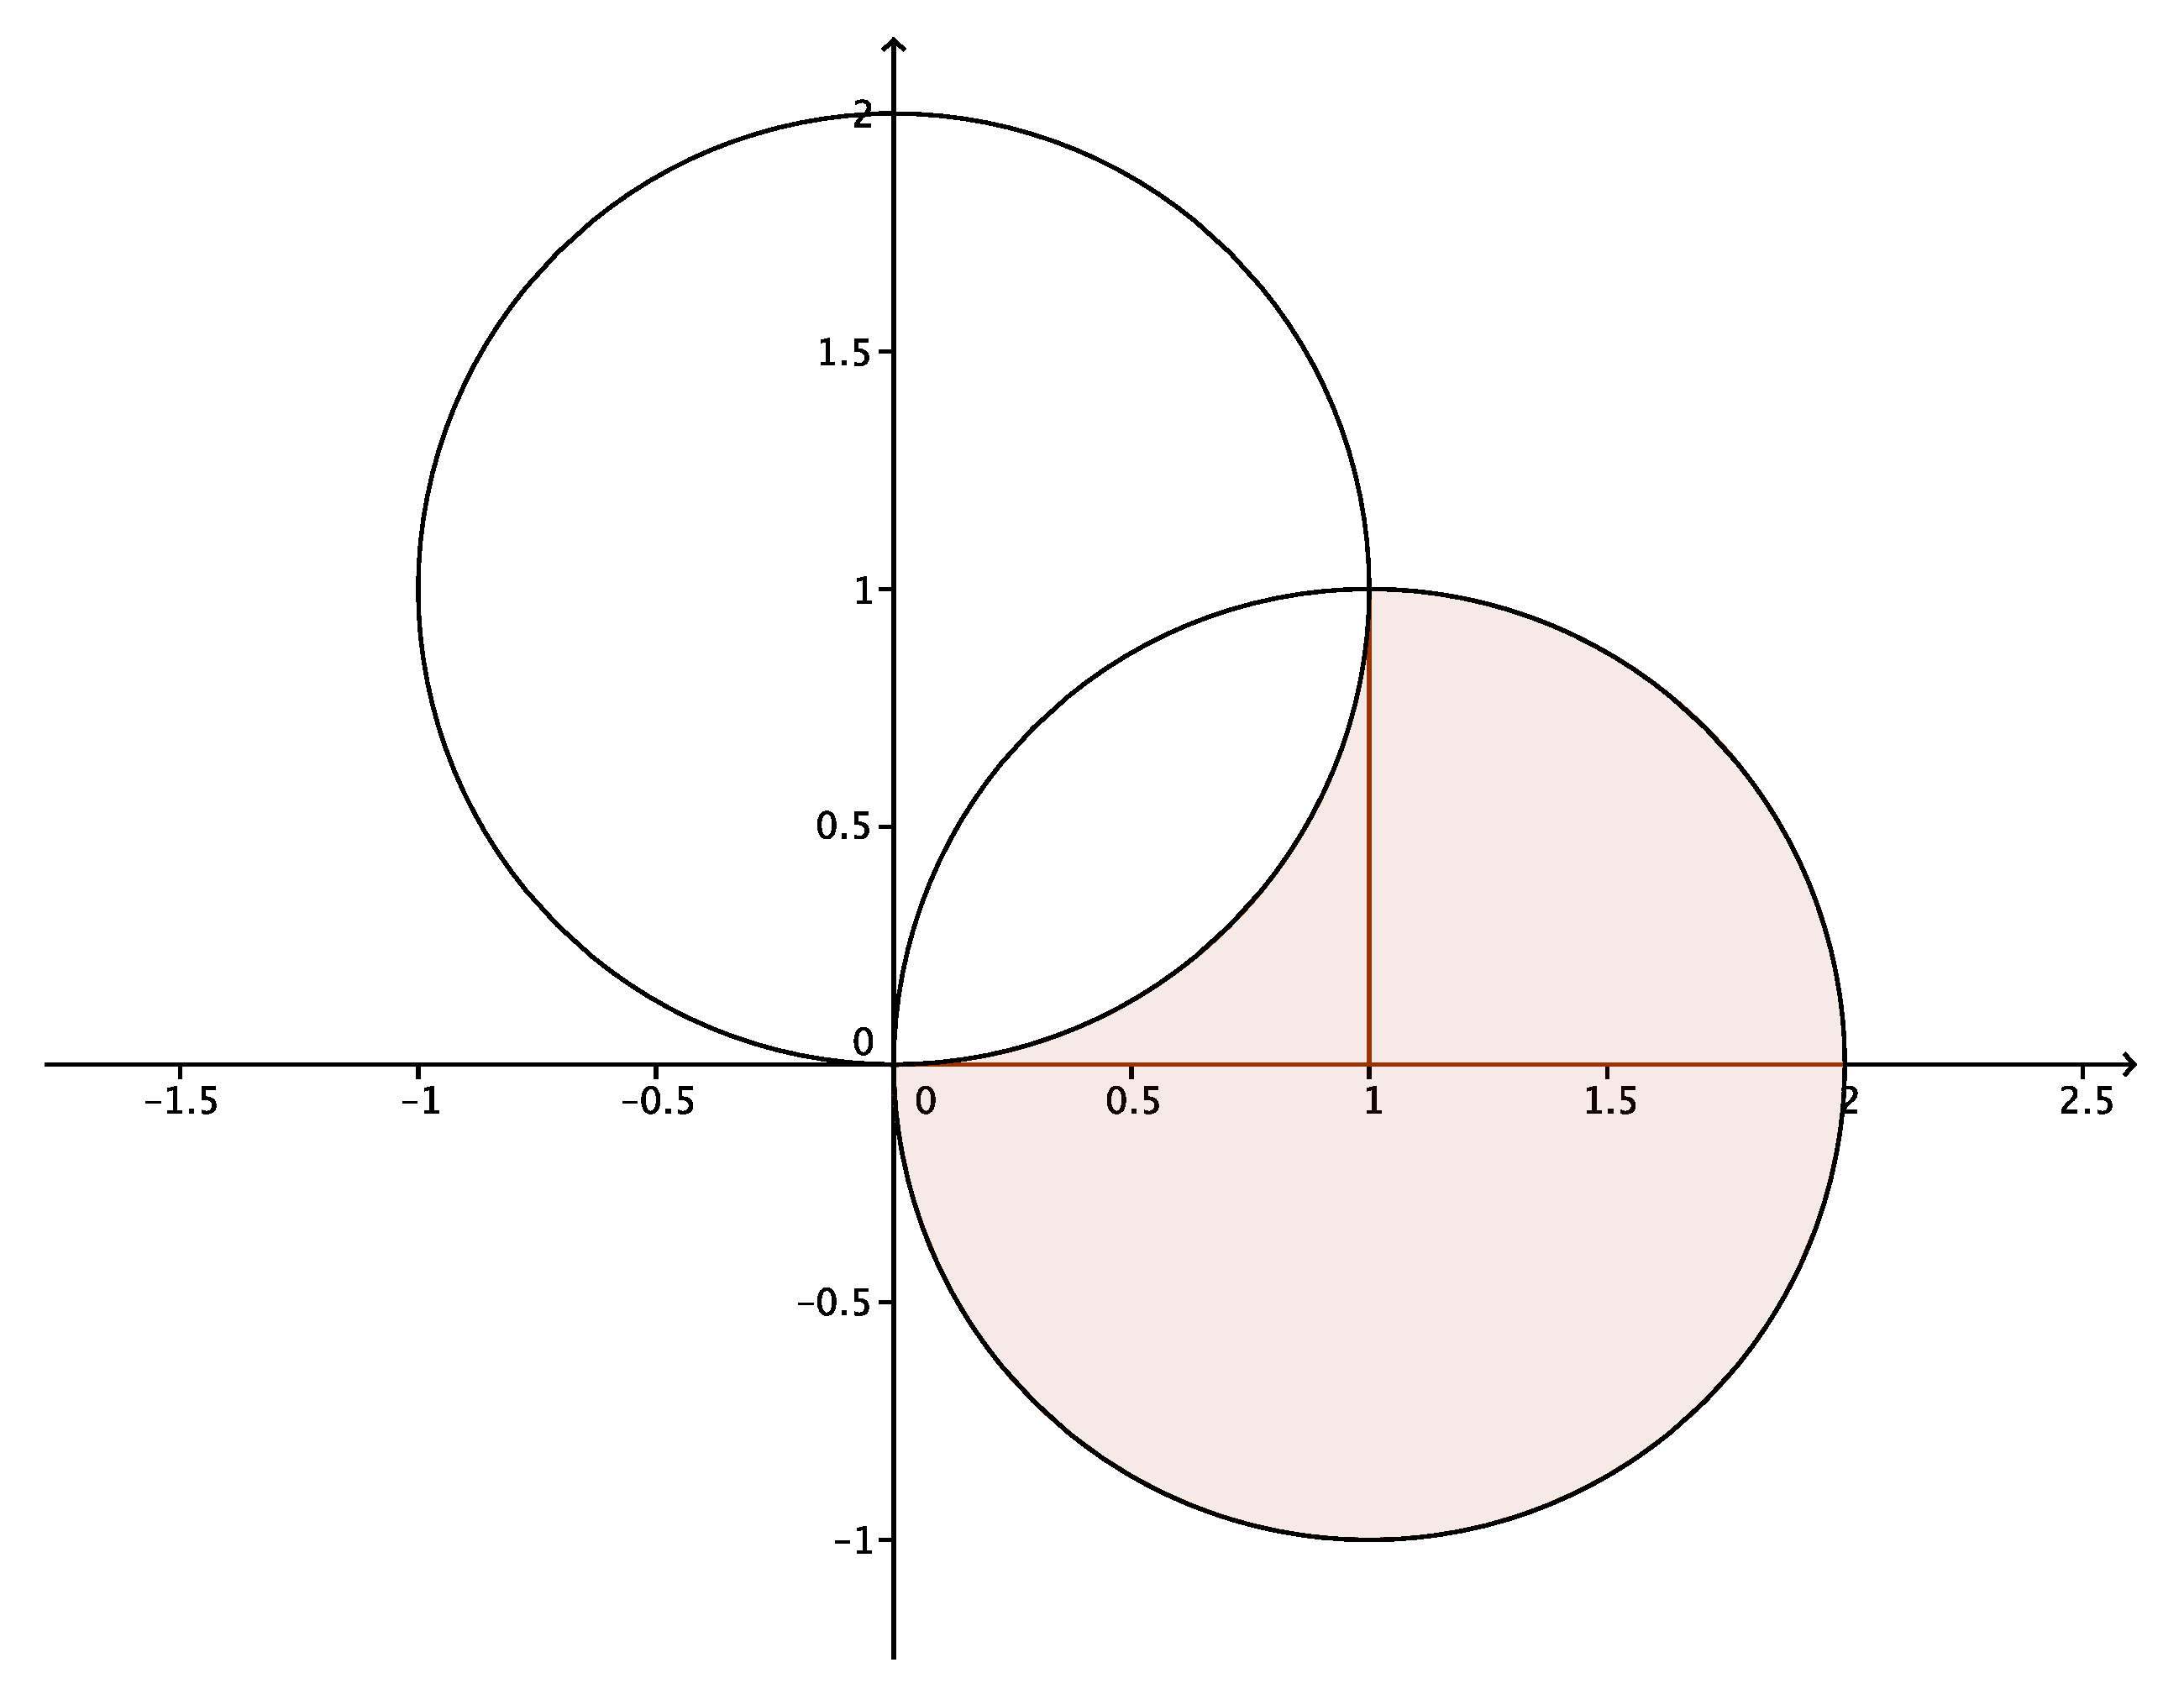
\includegraphics[width=0.6\textwidth]{WS6-4c}
\end{center}

The desired area consists of two parts: the half of the circle $r=2\cos\theta$ that lies below the $x$-axis, which has area $\pi/2$, and the part of this circle above the $x$-axis that is outside the circle $r=2\sin\theta$. Noting that the two circles intersect when $\theta=\pi/4$, this area can be computed by finding the area inside the circle $r=2\cos\theta$ for $0\leq \theta\leq \pi/4$, and subtracting the area that lies inside the circle $r=2\sin\theta$ on this same interval. Thus,
\begin{align*}
 A & = \frac{\pi}{2} + \frac{1}{2}\int_0^{\pi/4}((2\cos\theta)^2-(2\sin\theta)^2)\,d\theta\\
& = \frac{\pi}{2} + 2\int_0^{\pi/4}(\cos^2\theta-\sin^2\theta)\,d\theta\\
& = \frac{\pi}{2} + 2\int_0^{\pi/4}\cos(2\theta)\,d\theta\\
& = \frac{\pi}{2} + \sin(2\theta)\vert_0^{\pi/4} = \frac{\pi}{2}+1.
\end{align*}

 \item The area common to the inside of the curves $r=\cos\theta$ and $r=\sin(2\theta)$, in the first quadrant.

\begin{center}
 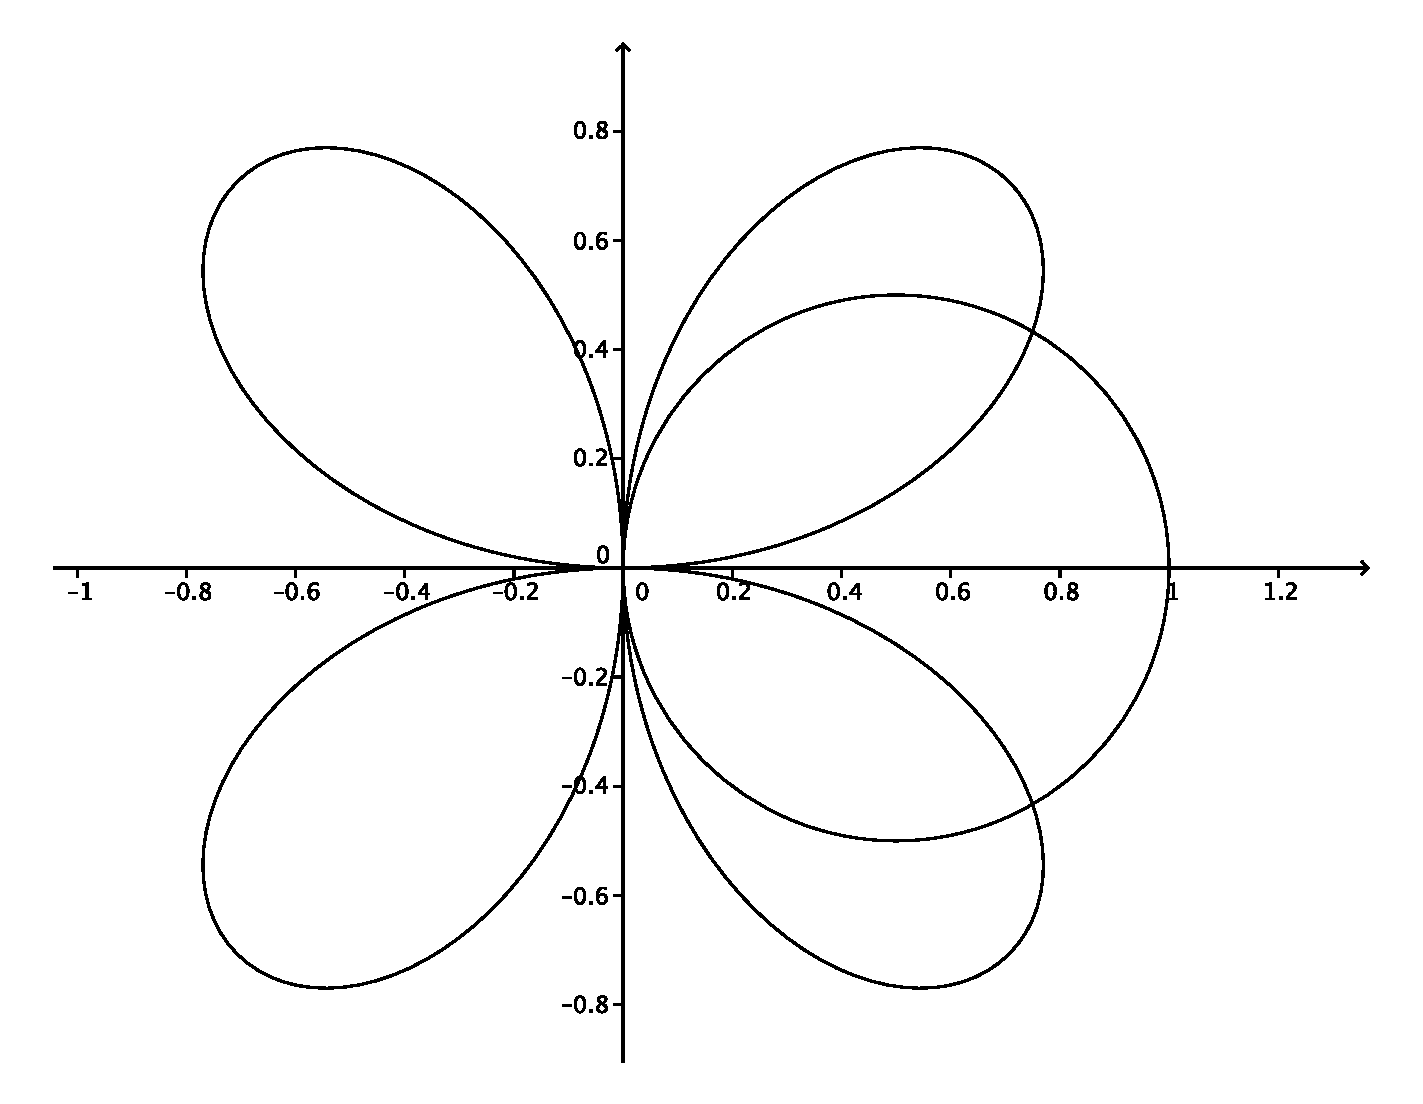
\includegraphics[width=0.6\textwidth]{WS6-4d}
\end{center}

The point of intersection between the two curves in the first quadrant occurs when $\theta = \pi/6$. From the diagram, we can see that the area common to the inside of the two curves can be described as follows:\\
For $0\leq \theta\leq \dfrac{\pi}{6}$, we have $0\leq r\leq \sin(2\theta)$.\\
For $\dfrac{\pi}{6}\leq \theta \leq \dfrac{\pi}{2}$, we have $0\leq r\leq \cos\theta$.

Thus, the area is given by
\begin{align*}
 A & = \frac{1}{2}\int_0^{\pi/6}\sin^2(2\theta)\,d\theta + \frac{1}{2}\int_{\pi/6}^{\pi/2}\cos^2\theta\,d\theta\\
& = \frac{1}{4}\int_0^{\pi/6}(1-\cos(4\theta))\,d\theta + \frac{1}{4}\int_{\pi/6}^{\pi/2}(1+\cos(2\theta))\,d\theta\\
& = \frac{\pi}{8}-\frac{3\sqrt{3}}{32}.
\end{align*}

\end{enumerate}
\end{enumerate}



\end{document}